\subsection{Wellenausbreitung mit bewegtem Sender/Empfänger} \enter
\subsubsection{Experiment: WWW mit bewegter Quelle}
\begin{center}
	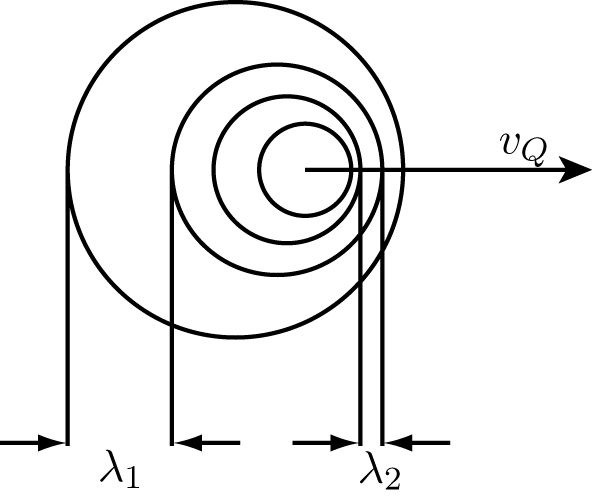
\includegraphics[width=0.5\linewidth]{skizzen/19/19B29}
\end{center}
Unterschied in $ \lambda $, je nachdem ob sich die Quelle zum Empfänger oder von ihm weg bewegt (Doppler-Effekt).\\
$ \Rightarrow $ Frequenzänderung $ \Delta\nu = \nu-\nu_0 $ Doppler-Verschiebung \\
\begin{align*}
\nu_0 &= \frac{1}{T_0} \text{ : Frequenz der ruhenden Quelle ($ \rightarrow $ Tropfen) }\\
v_Q &: \text{ Geschwindigkeit der Quelle }\\
v_{Ph} &: \text{ Phasengeschwindigkeit der Welle }\\
v_{Ph} &= \frac{\lambda_0}{T_0} = \nu_0 \cdot \lambda_0
\end{align*}
\begin{align*}
\nu_2'&=\frac{v_{Ph}}{\lambda_2} = \frac{v{Ph}}{(v_{Ph}-v_Q)\cdot T_0} = \frac{1}{1-\frac{v_Q}{v_{Ph}}} \cdot \nu_0 \overset{v_Q<<v_{Ph}}{=} (1+\frac{v_Q}{v_{Ph}}) \cdot \nu_0 \hspace{1cm}, \frac{1}{1-x} \overset{x<<1}{\approx} 1+x \\
\nu_1'&=\frac{v_{Ph}}{\lambda_1} = \frac{v{Ph}}{(v_{Ph}+v_Q)\cdot T_0} = \frac{1}{1+\frac{v_Q}{v_{Ph}}} \cdot \nu_0 \overset{v_Q<<v_{Ph}}{=} (1-\frac{v_Q}{v_{Ph}}) \cdot \nu_0
\end{align*}
\begin{align*}
\text{Alternativ: } &v_Q > 0 : \text{ Quelle } \rightarrow \leftarrow \text{ Empfänger } \Rightarrow \nu_2 = \nu_0\\
&v_Q<0: \text{ Quelle } \leftarrow \rightarrow \text{ Empfänger } \Rightarrow \nu_1<\nu_0
\end{align*}
\subsubsection{Bewegter Empfänger}
Bewegt sich E mit $ v_E $ , so wird die effektive Ausbreitungsgeschwindigkeit der Welle geändert:\\

(i) Q $ \rightarrow $ $ \leftarrow $ E :\\
$$ \nu'  = \frac{v_{Ph}+v_E}{\lambda_0} = \frac{v_{Ph}(1+\frac{v_E}{v_{Ph}})}{\lambda_0}=v_0(1+\frac{v_E}{v_{Ph}})$$\\
ist die Geschwindigkeit der Bewegung klein, so ist das Ergebnis für bewegte Quelle und bewegter Empfänger gleich.\\
Beides bewegt sich: 
\begin{center}
	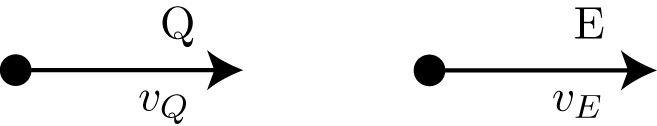
\includegraphics[width=0.3\linewidth]{skizzen/19/19B30}
\end{center}
\begin{align*}
\nu'=\frac{v_{Ph}-v_E}{v_{Ph}-v_Q} \cdot \nu \\
v_Q,v_E << v_{Ph}\\
\nu'=\frac{1-\frac{v_E}{v_{Ph}}}{1-\frac{v_Q}{v_{Ph}}} \cdot \nu &= \left[ (1-\frac{v_E}{v_{Ph}}) (1+\frac{v_Q}{v_{Ph}})  \right] \cdot \nu \\
&= [ 1-\frac{(v_E-v_R)}{v_{Ph}} - \frac{v_E \cdot v_Q}{\underbrace{v^2_{Ph}}_{\mathclap{\approx 0 \text{ (2.0rdnung)}}}}  ] \cdot \nu\\
\enter
v_E-v_Q&=v_{rel}\\
\nu'=&(1-\frac{v_{rel}}{v_{Ph}}) \cdot \nu
\end{align*}
$$ \underline{v_{rell} < 0: \hspace{5mm} Q\rightarrow\leftarrow E \Rightarrow \nu' > \nu} $$
Beispiel: Polizeisirene: $ v_{Ph} = \SI{300}{\meter\per\second} $ ; $ v_Q=\SI{30}{\meter\per\second} = \SI{110}{\kilo\meter\per\hour}$
$$ \Rightarrow \nu'=(1+10^{-1}) \cdot \nu \longrightarrow \nu' (1-10^{-1}) \cdot \nu $$
\kommentar{Ich denke hier ist irgendwas falsch im Skript, die zweite obige Gleichung ist gar keine Gleichung}
\HL
Unterschied zu elektromagnetischer Wellen: Lichtgeschwindigkeit ist konstant.\\
Grenzfall des Doppler-Effektes:
\begin{align*}
v_Q=v_{Ph}\\
\Rightarrow \lambda'=(v_{Ph} - v_Q) \cdot T_v = 0?\\
v_Q > v_{Ph}
\end{align*}
\begin{center}
	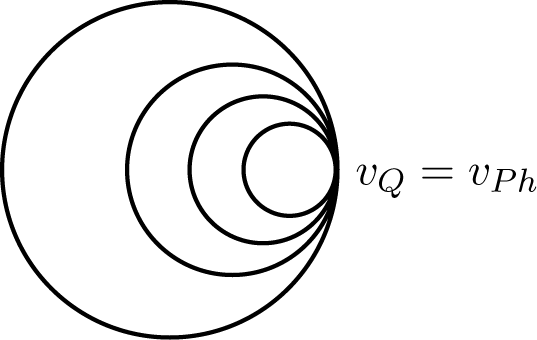
\includegraphics[width=0.4\linewidth]{skizzen/19/19B31}
\end{center}
\bild
Im Zeitraum $ t $:\\
Quelle bewegt sich um $ A $ nach $ B $ \hspace{1cm} $\overline{AB} = v_Q \cdot t$\\
Welle von $ A $ nach $ A' $ \hspace{1cm} $ \overline{AA'} = v_{Ph} \cdot t $
\enter
\underline{$ \alpha $: Öffnungswinkel} $ \sin\alpha = \frac{\overline{AA'}}{\overline{AB}} = \frac{v_{Ph}}{v_Q}$
\enter
2. Kreiswellen, emittiert zur Zeit $ t_2 $ : $ 0<t_2<t $
\begin{align*}
\sin\alpha = \frac{v_{Ph} (t-t_2)}{v_Q(t-t_2)} = \frac{v_{Ph}}{v_Q}
\end{align*}
für $ v_Q>v_{Ph} $: Die Einhüllende der Wellenfronten ist ein Kegel mit Öffnungswinkel $ \underbracket{\alpha}_{\mathclap{\sin\alpha=\frac{v_{Ph}}{v_Q}}} $ (Mach-Kegel)\\
$ \Rightarrow $ Dort akkumuliert sich eine Große Gesamtamplitude \\
$ \Rightarrow $ Diese Einhüllende folgt der Quelle mit Zeitversatz\\
\enter
$ \Rightarrow $ Schall:
\bild
Zusätzlich "Wolkenscheibeneffekt"
Adiabatische Expansion nach starker Kompression $ \Rightarrow $ Reduzierung der Temperatur\\
Bei hoher Luftfeuchtigkeit: Taubildung an Mach-Kegel-Spitze!
\bild